
\chapter{Block recognition}\label{ch:block_recognition}

In order to complete the block recognition part of our project, we had to go through 3 main steps, the background substraction, color and edge detection.

\section{Background substraction}

\section{Color detection}

 	Once the background substracted, we obtained the color of the blocks experimentaly by using the tool 'Pixel region' in Matlab. A color can be expressed with values between 0 and 255 for its primary colors, red, green and blue. Thus, for each block, we placed the 'Pixel region' tool on it to get a range for the RGB parameters.\par
\begin{flushleft}
Let's take an example with the yellow block.
\end{flushleft} \par

\begin{figure}[hb]
  \centering
  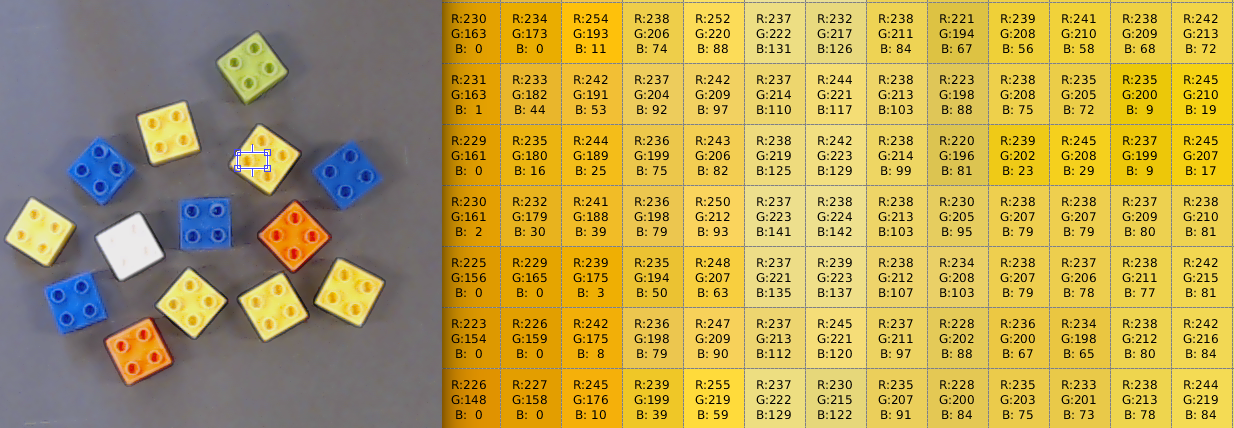
\includegraphics[scale=0.3]{figures/Thres_Y_manualy2.png}
  \caption[LABEL] {CAPTATION TEXT}
\end{figure}

Here the result by experiment gives us more or less a range of R = [], G = [] and B = [] for the RGB parameter. This parameter is then used to check in a loop that every pixel of the image are within the ranges.\par
In the image below the pixels being in the RGB parameter are highlighted in white while the others are put into black. 

\begin{figure}[hb]
  \centering
  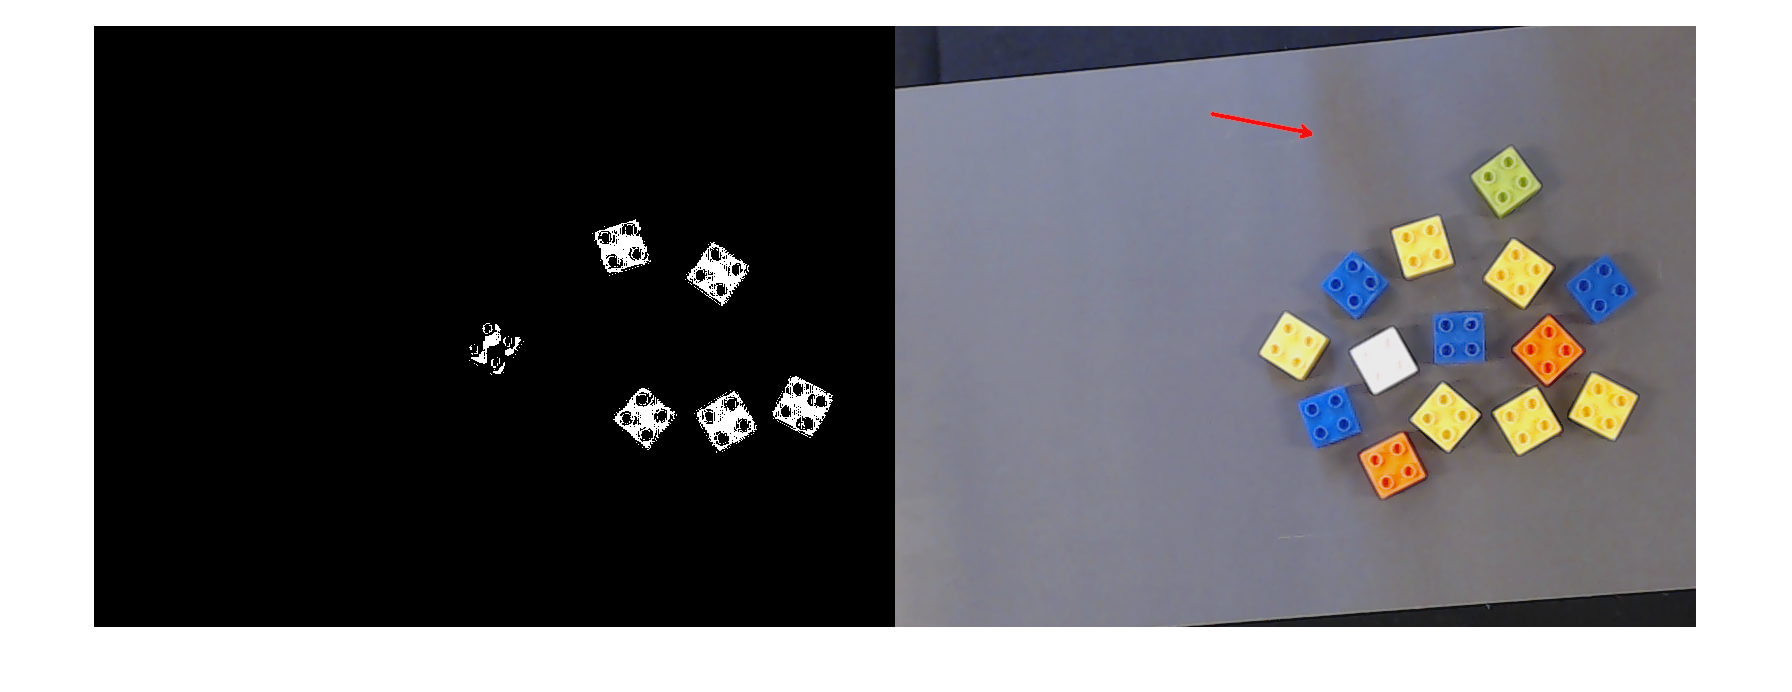
\includegraphics[scale=0.3]{figures/Thres_Y_bad2.png}
  \caption[LABEL] {CAPTATION TEXT}
\end{figure}
  
\begin{flushleft}
We can see that the 6 yellow blocks are detected. However, the one on the left is partially detected. This is the consequence of the different lights in the robot cell. The RBG range was define on a block placed in a zone of shadow (see the red arrow on the picture).
\end{flushleft}  
\par

\begin{flushleft}
Thus, the color recognition was redefined taking into account the different light inside the robot cell. All the yellow blocks are now detected.
\end{flushleft}


\begin{figure}[hb]
  \centering
  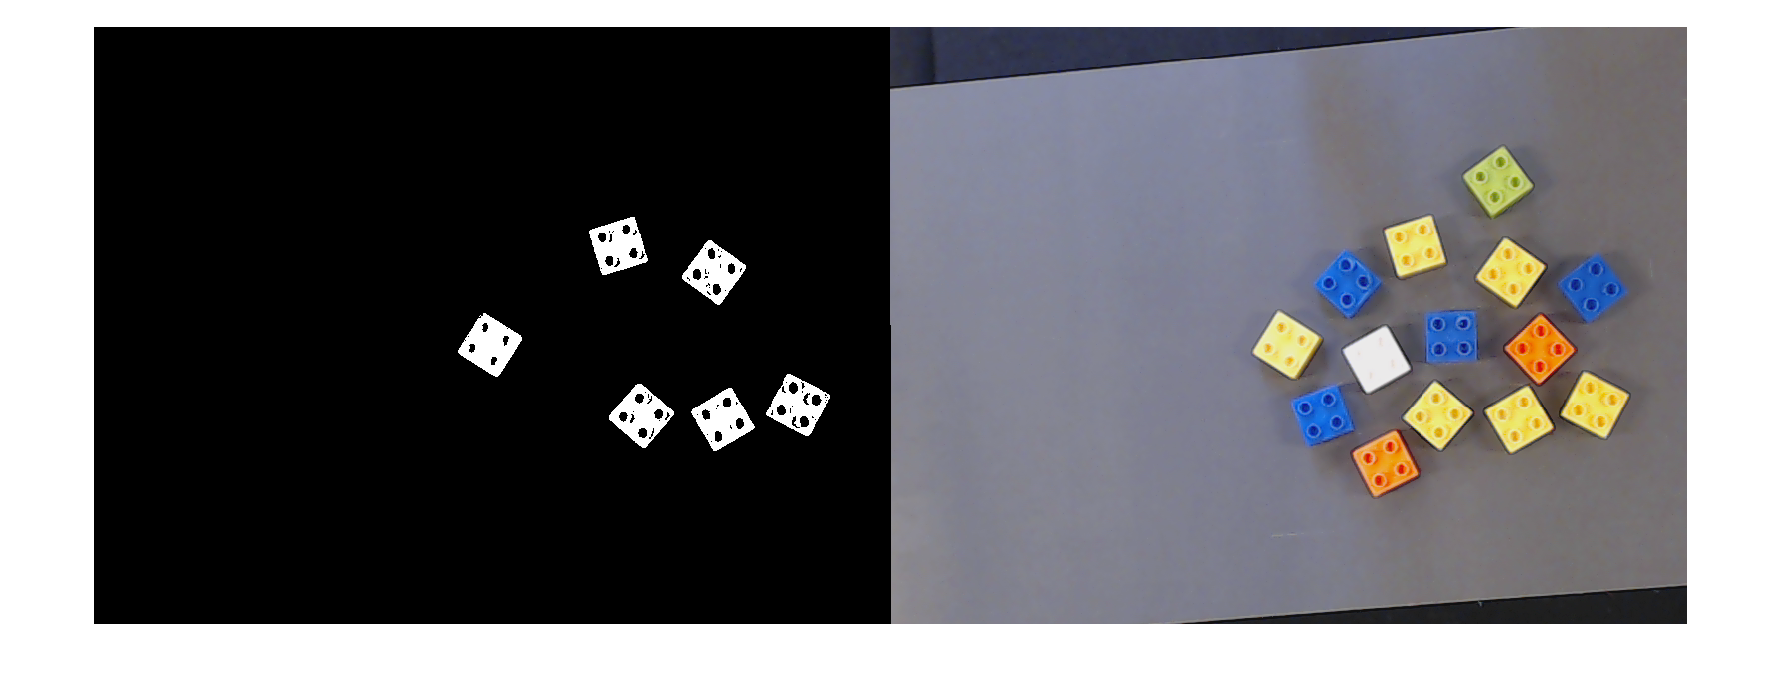
\includegraphics[scale=0.3]{figures/Thres_Y_good.png}
  \caption[LABEL] {CAPTATION TEXT}
\end{figure}

\begin{flushleft}
An other solution would have been to set up a source of light inside the cell to have more precise ranges for the colors resulting in more robust system.
\end{flushleft}



 \section{Edge detection}

	There is different methods to detect the edges in an image. To pick the best one for our application, we played around the Canny, log, Prewitt, Roberts, Sobel and zerocross methods and their parameters as the threshold, direction and the standard deviation of the filter. \par

 \begin{flushleft}
	We chose to detect the edges based on the resulting image of the color recognition. Below can be seen the color recognition of the blue blocks.
 \end{flushleft}

	\begin{figure}[hb]
  \centering
  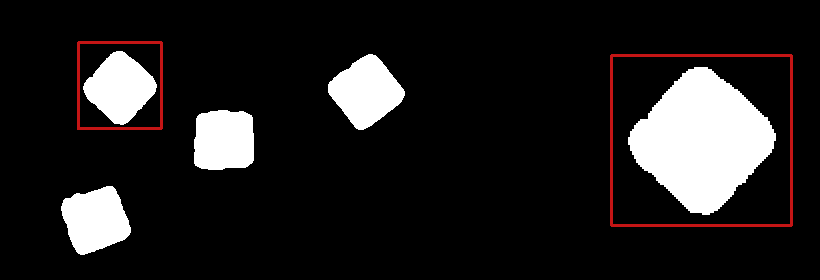
\includegraphics[scale=0.3]{figures/color_rec_zoom.png}
  \caption[LABEL] {CAPTATION TEXT}
\end{figure}	
	

 \begin{flushleft}
As seen on the picture above, the shapes of the blocks that we get from the color recognition are irregular and so will be the edges. Thus, we used the Canny method that allows us to choose a stantard deviation of its filter in order to smooth the irregularities of the shapes.\par 
 \end{flushleft}

\begin{flushleft}
The default value of the deviation is $\sqrt{2}$, increasing the deviation will result in smoother lignes until getting a round shape.
\end{flushleft}

	\begin{figure}[hb]
  \centering
  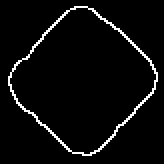
\includegraphics[scale=0.5]{figures/Canny_sqrt2.png}
  \caption[LABEL] {CAPTATION TEXT}
\end{figure}	
  	\begin{figure}[hb]
  \centering
  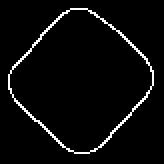
\includegraphics[scale=0.5]{figures/Canny_4.png}
  \caption[LABEL] {CAPTATION TEXT}
\end{figure}	
  	\begin{figure}[hb]
  \centering
  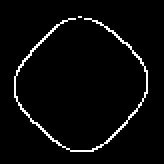
\includegraphics[scale=0.5]{figures/Canny_10.png}
  \caption[LABEL] {CAPTATION TEXT}
\end{figure}	
  	\begin{figure}[hb]
  \centering
  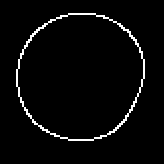
\includegraphics[scale=0.5]{figures/Canny_25.png}
  \caption[LABEL] {CAPTATION TEXT}
\end{figure}	
	

As a result of the tests done, we chose to use the Canny method with a standard deviation of 4, giving us smoother lignes but not too round corners in order to calculate its position.


\begin{flushleft}
 block reconstruction ?
 \end{flushleft}